%全体の2段組.tex 

% どちらでも確認
\documentclass[twocolumn,10pt]{jarticle} 
% \documentclass[twocolumn,10pt]{jreport}

\usepackage{listings,jlisting}
\usepackage[dvipdfmx]{graphicx,color}
\usepackage{eclbkbox}
\usepackage{forloop}
\usepackage{url}

\usepackage{bxwareki} % 令和対応

\newcommand{\zr}{$\rightarrow$}

\setlength{\columnsep}{3zw} 
\title{\TeX 改造} 
\author{i13302} 
\date{\warekitoday}

%%==== ソースコードのレイアウト
\lstset{%
	language=C,
	breaklines=true,%改行
	numbers=left,%
	numberstyle={\scriptsize},%
	stepnumber=1,
	numbersep=1zw,%
	lineskip=-0.5ex,%
	basicstyle=\ttfamily\footnotesize\fontsize{8}{8},
	frame=single,%
	columns=[l][l]{fullflexible},
	tabsize=4,
	xleftmargin=3zw,
	xrightmargin=3zw, % 最所先生オリジナル
	framexleftmargin=3zw, %ソースの左枠に行番号
	commentstyle={\ttfamily \color[rgb]{0,0.5,0}},
	keywordstyle={\bfseries \color[rgb]{1,0,0}},
	stringstyle={\ttfamily \color[rgb]{0,0,1}},
	literate= %特殊文字
		*{\#include}{{\textcolor[rgb]{0.7,0.3,0.5}{\#include}}}{7}
		 {\#define} {{\textcolor[rgb]{0.7,0.3,0.5}{\#define}}}{6}
		 {\#if}     {{\textcolor[rgb]{0.7,0.3,0.5}{\#if}}}{2}
		 {\#else}   {{\textcolor[rgb]{0.7,0.3,0.5}{\#else}}}{4}
		 {\#endif}  {{\textcolor[rgb]{0.7,0.3,0.5}{\#endif}}}{5}
		 {\#elif}   {{\textcolor[rgb]{0.7,0.3,0.5}{\#elif}}}{4}
		 {\#ifndef} {{\textcolor[rgb]{0.7,0.3,0.5}{\#ifndef}}}{6}
		 {\#ifdef}  {{\textcolor[rgb]{0.7,0.3,0.5}{\#ifdef}}}{5},
}


%%%%%%    TEXT START    %%%%%% 
\begin{document} 
\maketitle 
\section{はじめに}
\TeX はスタンフォード大学教授(数学)D.E.Knuth(1938~)による文書整形システムです\cite{TeX入門}.
Dockerにすることで,柔軟にキメラな \TeX 環境を作成できます.
\par 
aboutstyディレクトリにstyファイルを配置すると,Docker build時に読み込みます.

\section{コンパイル}
同梱のmptex2pdfスクリプトにより,3回通るようにしています.
引数を2つ指定すると,bibtex対応でコンパイルします.

\section{URL表示}
urlパッケージを導入しています.\url{https://google.com}.

\section{ソースコード表示}
指導教員にお願いして,行番号に枠を入れました.

\begin{lstlisting}[caption=FORMURAの定義]
#define FORMULA  0 // 途中経過を表示
\end{lstlisting}

\lstinputlisting[caption=カラツバ法を実行 bignum\_kara()]{./src/bignum_kara.txt}

\section{令和対応}
TeX LiveがVer 2017なので,BXwarekiパッケージ\cite{bxwareki}にて,対応しています.

\begin{enumerate}
	\item ``\textbackslash\textbackslash  today'' \zr \today
	\item ``\textbackslash\textbackslash warekitoday'' \zr \warekitoday
\end{enumerate}

\section{参考文献/関連図書}
bibtexにて,``junsrt.bst''ファイルを改修しています.
\begin{enumerate}
	\item ``@misc''表示の際に,url前に改行
	\item 日付は年のみ表示
	\item ``@bachelorthesis''にて,学士論文に対応
	\item ``Master's thesis'' \zr ``修士論文''
\end{enumerate}

\subsection{epsファイル}
昔懐かしのepsファイルにも対応しています(図\ref{fig:epsSample}).
\begin{figure}[htbp]
	\centering
	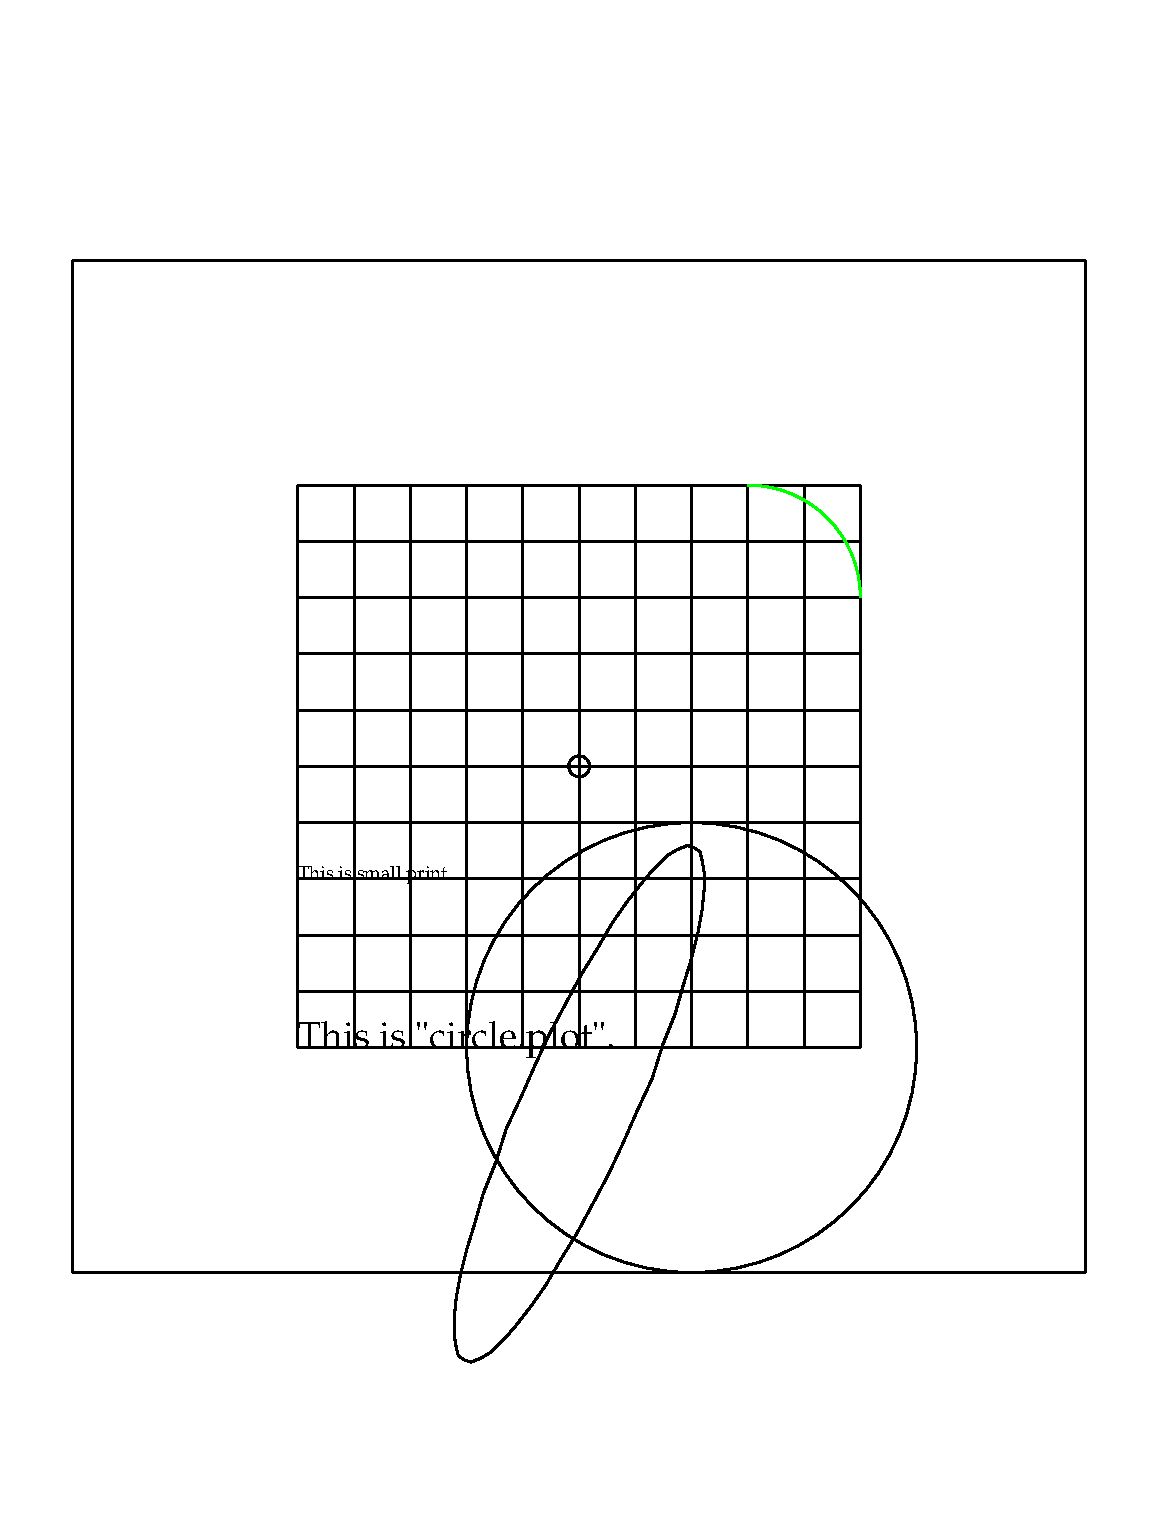
\includegraphics[width=6cm]{./fig/circle.eps}
	\caption{epsSample\cite{EPSFiles}}
	\label{fig:epsSample}
\end{figure}


\bibliography{bibtex} % 参考文献
\bibliographystyle{junsrt}

\end{document}
